\setcounter{step}{0}
%------------------------------------------
% information doc
\subsection{Salko krém na tortu}
\PrepTime{10}
\CookingTime{0}
\CookingTempe{0}
\TypeCooking{Mixovanie}
\NbPerson{4}
\Image{0 0 400 400}{images/pistkot_krem_salko} %style 2
%------------------------------------------

\begin{ingredient}
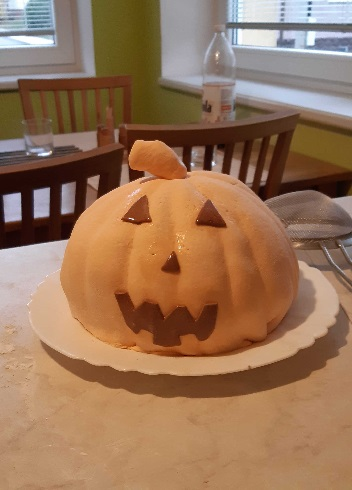
\includegraphics[height=5.5cm]{images/pistkot_krem_salko}
\def\portions{4}%
\textbf{{\normalsize Ingrediencie (\portions porcie):}}
%\vspace{0.5cm}
\begin{main}
	\item 250g maslo
	\item 1 konzerva uvareného salka
\end{main}
\end{ingredient}
\begin{recipe}
\textbf{{\normalsize Príprava:}}
\begin{enumerate}


\item{Maslo vyložíme z chladničky a necháme zmäknúť.}
\item{Maslo mixujeme a popri tom po lyžiciach pridávame salko}


\end{enumerate}
\end{recipe}

\begin{notes}

\end{notes}
\clearpage	